% $Id: 20041109.tex 367 2004-11-23 10:22:38Z conall $

\documentclass[a4paper,12pt]{article}

\usepackage{graphicx}

\setlength{\parindent}{0mm}
\setlength{\parskip}{7.5mm}

\begin{document}

\bibliographystyle{ieeetr}

\title{Course 3BA5: Computer Engineering \\ Assignment 2 \\ Pipelining
Techniques in the \\ IBM PowerPC 970 (A.K.A PowerPC G5)}

\author{Conall O'Brien \\ conallob@maths.tcd.ie \\ 01734351}

\maketitle

\begin{figure}[hb]

\begin{center}

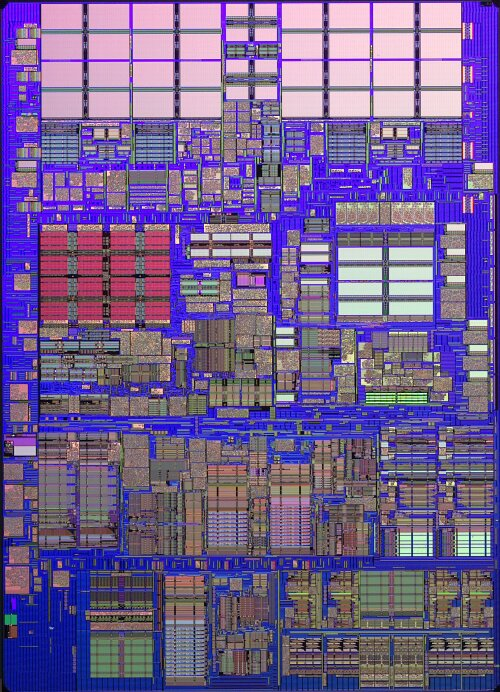
\includegraphics{powerpc970-1.png}

\end{center}

\caption{\cite[The IBM PowerPC 970 Microprocessor Unit]{a10}}

\end{figure}

\tableofcontents

\section{Overview}

\section{The PowerPC Architecture}

\cite[In 1991]{a3}, Apple, IBM and Motorola formed the AIM alliance to
produce a competitor to the Windows Operating System on the Intel x86
architecture. The PowerPC architecture is the sole surviving product of
this alliance.


The PowerPC architecture is a \cite[RISC based]{a3} architecture with
great potential which was has gained a market share in the desktop
computing market as the nearest competitor to the Intel x86
architecture, despite \cite[troubles experienced by numerous PC
manufactures, such as IBM]{a3} in creating a PowerPC based
systems.


To date, the PowerPC architecture is commonly used in all Apple
Macintosh systems, both desktop and server, as well as in high
performance servers from IBM. Recent developments have also seen the
PowerPC become an embedded processor, used in embedded devices such as
\cite[the Nintendo CameCube, the Microsoft Xbox 2, Cisco dedicated 
networking hardware, and the TiVo set top box.]{a3}. An extremely high
performance CPU, called the \cite[Cell Technology]{a3}, being developed for
embedded devices, is also a member of the PowerPC architecture.

\subsection{The PowerPC 970}

The PowerPC 970 is the most recent member to the AIM (Apple, IBM,
Motorola) Consortium's PowerPC architecture commonly found in many 
systems, such as Apple Macintosh computers and various high 
performance systems. One major difference between the PowerPC 970 and other 
members of the PowerPC architecture family is it's 64 bit design, 
giving it significant 64 bit based benefits which include an 
increased memory addressing beyond the 32bit CPU limit of 4GB and 
the reduction of steps when computing high precision computations 
using multiple registers for single operands, as explained
\cite[here]{a6}


The PowerPC 970 has been designed primarily for high performance
workstation and computation roles, particularly for operations involving
a high degree of precision using custom written computational software
which can be optimized to take full advantage of the PowerPC 970 64 bit
data-path pipeline and 64 bit registers. Hence why in November 2004, the
\cite[published list of high performance computing systems]{a11} lists
two PowerPC 970 based systems in the top 10, namely the \cite[Marenostrum
in the Barcelona Supercomputer Centre and the System X system in
Virginia Tech]{a11}.

\begin{figure}[hb]

\begin{center}

\scalebox{0.5}{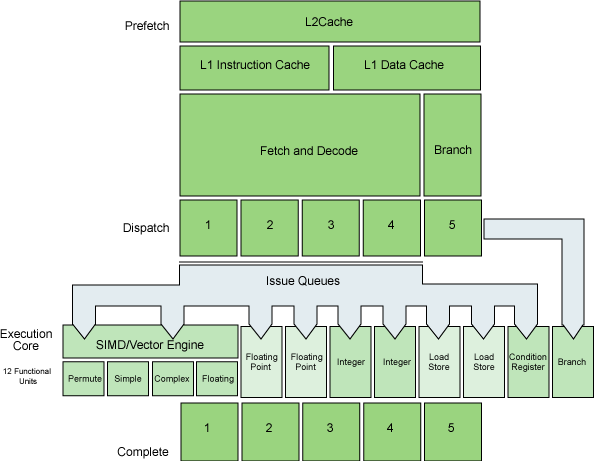
\includegraphics{970-arch.png}}

\end{center}

\caption{\cite[The IBM PowerPC 970 Microprocessor Design Layout]{a6}}

\end{figure}

\section{The Pipeline}

\subsection{Main Pipeline}

The PowerPC 970 has \cite[12 seperate execution cores]{a5}, including 
twin floating point cores, a sophisticated, multi execution core vector 
processing unit, dual integer units as well
as load/store, conditional register and branch units. Combined with this
wide execution core, is a long pipeline with over 
\cite[100 execution slots]{a1} and the ability to \cite[support 215
instructions (in various execution stages) in flight]{a5}, forming a wide 
and deep pipeline with mixed results.


Such a wide and deep pipeline has a few positive and negative features.
The main one being that the PowerPC 970 is capable of very high
performance computing as a result of the deep pipeline, yet it is also
flexible enough for many workstation uses with it's wide execution core.
However, in practice, such a pipeline will rarely be optimally used and
will likely include occasional pipeline stalls when converting from wide
pipelined tasks to narrow pipelined tasks in a short time frame.


To accompany the wide and deep pipeline of the PowerPC 970, are two
large caches. The L1 cache has two components, a \cite[64kb directly
mapped]{a1} instruction cache and a \cite[32kb 2 way assocciative]{a1}
data cache. Combined with the \cite[512KB L2 Cache]{a2}, the PowerPC 970
is able to fetch up to \cite[8 instructions per clock cycle]{a5} allowing
it to support \cite[fetching of upto 8 prefetch data streams]{a2}.

\subsubsection{Execution Cores}

\subsubsection{Integer Unit}

As \cite[discussed in detail]{a2}, the Integer Units in the PowerPC 970 are not
completely symmetric, thus conditional logic is used to ensure 
most integer operations are handled by one core and integer division 
and SPR operations are handled by special hardware when required.


As a result, the Integer performance of the PowerPC 970 is less than desirable
in situations requiring frequent complex operations. Both integer units
feature 64 bit registers, so in the future when pure 64 bit software is
more common, the full potential of native 64 bit compatible integer
registers will be unleashed, however, at present, very few non custom
written, high performance software utilizes this feature of the integer
units of the PowerPC 970.
 
\subsubsection{Floating Point Unit}

With \cite[80 registers, (32 PowerPC architectural registers and 48
rename registers)]{a2} in both of the PowerPC 970's floating point units, the
floating point execution core is completely pipelined for all floating
point operations bar floating division. 


Another \cite[well renoweded feature]{a5} of the PowerPC 970's floating
point functionality is it's ability to perform a "fused multiply-add"
operation, allowing the multiplication of two floating point numbers and
the addition of a third floating point number combined in a single
opcode operation. Although this operation is quite specialized and not
commonly utilized except using highly optimized machine code, the resulting
performance saves additional branch and arithmetic operations. 


Yet \cite[another key feature]{a2} the PowerPC 970 floating point execution core 
has the availability to perform certain floating point operations in
hardware decoding, without the need to decode such operations into
internal PowerPC RISC based architecture opcodes.


Due to the highly regarded reputation of the recent PowerPC family
members, particularly the PowerPC 7xxx series (also called the PowerPC
G4, primarily by Apple) prior to the PowerPC 970 series, the PowerPC 
CPU line has gained a well deserved name 
for floating point performance. The fully 64 bit pipeline of both 
floating point execution units in the PowerPC 970 and the ability to fuse 
floating point multiplication and addition of floating point numbers in 
one operation greatly enhance the floating point operation performance as 
well as the already well established reputation of the floating point high 
performance. 

\subsubsection{Vector Unit}

The PowerPC 970 was a \cite[128 bit vector processing unit (called the
Velocity Engine by Apple Computers)]{a5}, consisting of multiple
execution cores, using a sophisticated queue system and uses SIMD
(Single Instruction, Multiple Data) processing.


The sophisticated queuing system and multiple vector execution cores in
the PowerPC 970 is known as \cite[VMX (or AltiVec, Motorola's
trade marked term)]{a2}, which is currently only available to the PowerPC
970. The four execution cores within the vector unit each have specific
functions, \cite[one permute unit, one simple integer unit, one complex
integer unit and one floating point unit.]{a2}. These four execution
cores are all connected to \cite[a register file containing thirty two
128 bit precision architectural registers and sixteen rename
registers]{a2}.

\subsubsection{Load/Store Units}

The PowerPC 970 has \cite[dual load/store units for the entire CPU]{a1}, 
which are used to feed data both into and out of the data path pile-line, the L1 and 
L2 caches, as well as the main system memory.

\subsubsection{Conditional Register Unit}

The \cite[32 bit conditional register unit]{a6} is used by the PowerPC
970 to store meta data on \cite[integer and floating point]{a6} operands.
It can hold up to \cite[8 condition codes]{a6} which can be used to
describe the outcome of \cite[8 different instructions]{a6} for any of
the other execution cores in the PowerPC 970.

\subsubsection{Branch Prediction Unit}

In order to fully utilize the deep pipeline of the PowerPC 970, there is
a significant branch prediction unit dedicated to reducing the number of
pipeline stalls, maximizing efficiency. The branch prediction unit uses
2 prediction schemes, the first uses a \cite[16384 (16k) branch history 
table (BHT)]{a2} and a \cite[branch target buffer (BTB)]{a2}. 


The second scheme uses a \cite[global prediction table]{a2}, which has
another \cite[16k entry table]{a2} and each entry is associated with an
11 bit vector used to record the last 11 steps of the last 11 fetch
groups.

To merge both schemes together and to decide which scheme to use at any
given point, there is a third \cite[16k entry table, the selector table]{a2} 
which used at the front end to record which scheme works better for each 
branch. After a branch has been evaluated, the successes of both schemes
is recorded in the selector table.

\section{Conclusions}

The PowerPC 970 has high performance capabilities in certain high end
roles, making full use of it's deep and wide pipeline and accompanying
specialiased execution cores.


For ordinary desktop computing and certain integer computation, the
PowerPC 970 is less than ideal, however certain optimizations at compile
time are able to alleviate such problems.


It's main strengths lie with it's floating point and vector processing
cores, which out-perform all other members of the PowerPC architecture and
various other architectures, hence making it desirable for high end, high
precision number crunching. It is no wonder why two of the current top
10 supercomputers in the world are running PowerPC 970 CPUs.

\bibliography{PowerPC970}

\end{document}
